\documentclass[10pt,landscape]{article}

\usepackage[utf8]{inputenc}
\usepackage[T1]{fontenc}
\usepackage[paperwidth=24in,paperheight=15in,margin=0.45in]{geometry}
\usepackage{amsmath,amssymb,amsfonts}
\usepackage{booktabs}
\usepackage{graphicx}
\graphicspath{{./}{../}}
\usepackage{multicol}
\usepackage{xcolor}
\usepackage{caption}

\definecolor{stanfordred}{HTML}{8C1515}
\definecolor{navyheader}{HTML}{1F3A60}

\captionsetup{font=small,labelfont=bf,skip=3pt}
\setlength{\columnsep}{0.35in}
\setlength{\parindent}{0pt}
\setlength{\parskip}{4pt}
\pagestyle{empty}

\begin{document}

\begin{center}
  {\colorbox{stanfordred}{\parbox{0.99\textwidth}{\centering\vspace{0.12in}
    {\Huge\bfseries\color{white} VEHICLE SPEED ESTIMATION WITH OPTICAL FLOW AND LINEAR REGRESSION}\\[0.08in]
    {\Large\color{white} Computer Vision Track (Application \& Feature-Engineering Project)}\\[0.04in]{\normalsize\color{white}\texttt{https://github.com/Lukeeffs/vehicle-speed-optical-flow}}
  \vspace{0.12in}}}}
\end{center}

\vspace{0.08in}

\begin{multicols}{3}

\section*{\textcolor{navyheader}{1. Problem \& Ground-Plane Kinematics}}
\begin{itemize}
  \item \textbf{Goal:} Estimate ego-vehicle speed $\hat{v}_t \in \mathbb{R}_{\ge 0}$ ($\text{m/s}$) from $20\text{ Hz}$ monocular dashcam frames $(I_{t-1}, I_t)$ on CPU without wheel encoders, GPS, or LiDAR.
  \item \textbf{Pinhole Road Flow Law:} For camera height $H_c$, focal length $f$, and horizon $y_0$:
  $$\dot{y}(x,y,t) = \frac{(y - y_0)^2}{f H_c} v_t + f\omega_{\text{pitch}}(t), \quad \dot{x}(x,y,t) = \frac{(x - x_0)(y - y_0)}{f H_c} v_t$$
  \item \textbf{Leakage-Free Protocol:} Contiguous $70\%/15\%/15\%$ split ($5$-frame embargo). Random 5-fold CV leaks adjacent $50\text{ ms}$ frames ($0.4045$ vs.\ $0.5027\text{ m}^2/\text{s}^2$).
\end{itemize}

\begin{center}
  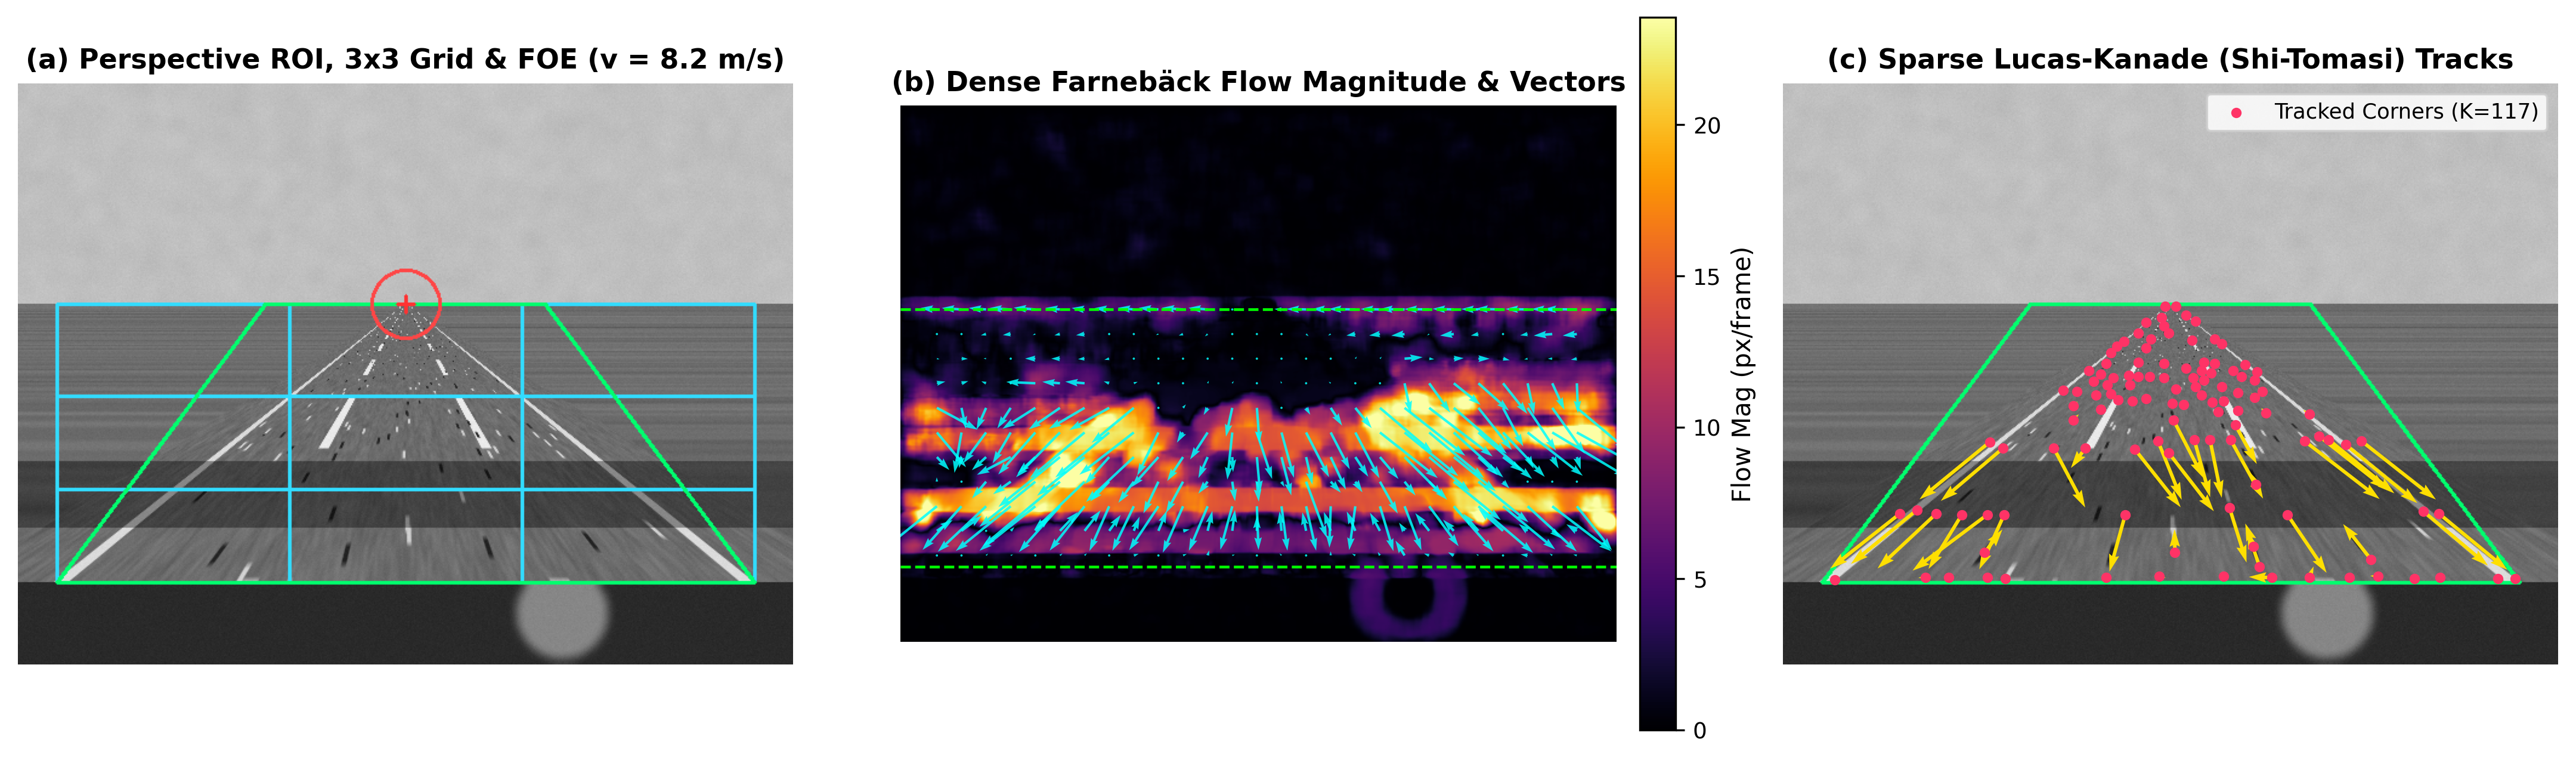
\includegraphics[width=0.98\linewidth]{figures/fig1_pipeline_and_roi_flow.png}
  \captionof{figure}{Trapezoidal ROI mask, $3\times 3$ perspective grid, FOE exclusion ($R=28\text{ px}$), Dense Farneb\"{a}ck heatmap, and Sparse Lucas-Kanade tracks.}
\end{center}

\begin{center}
  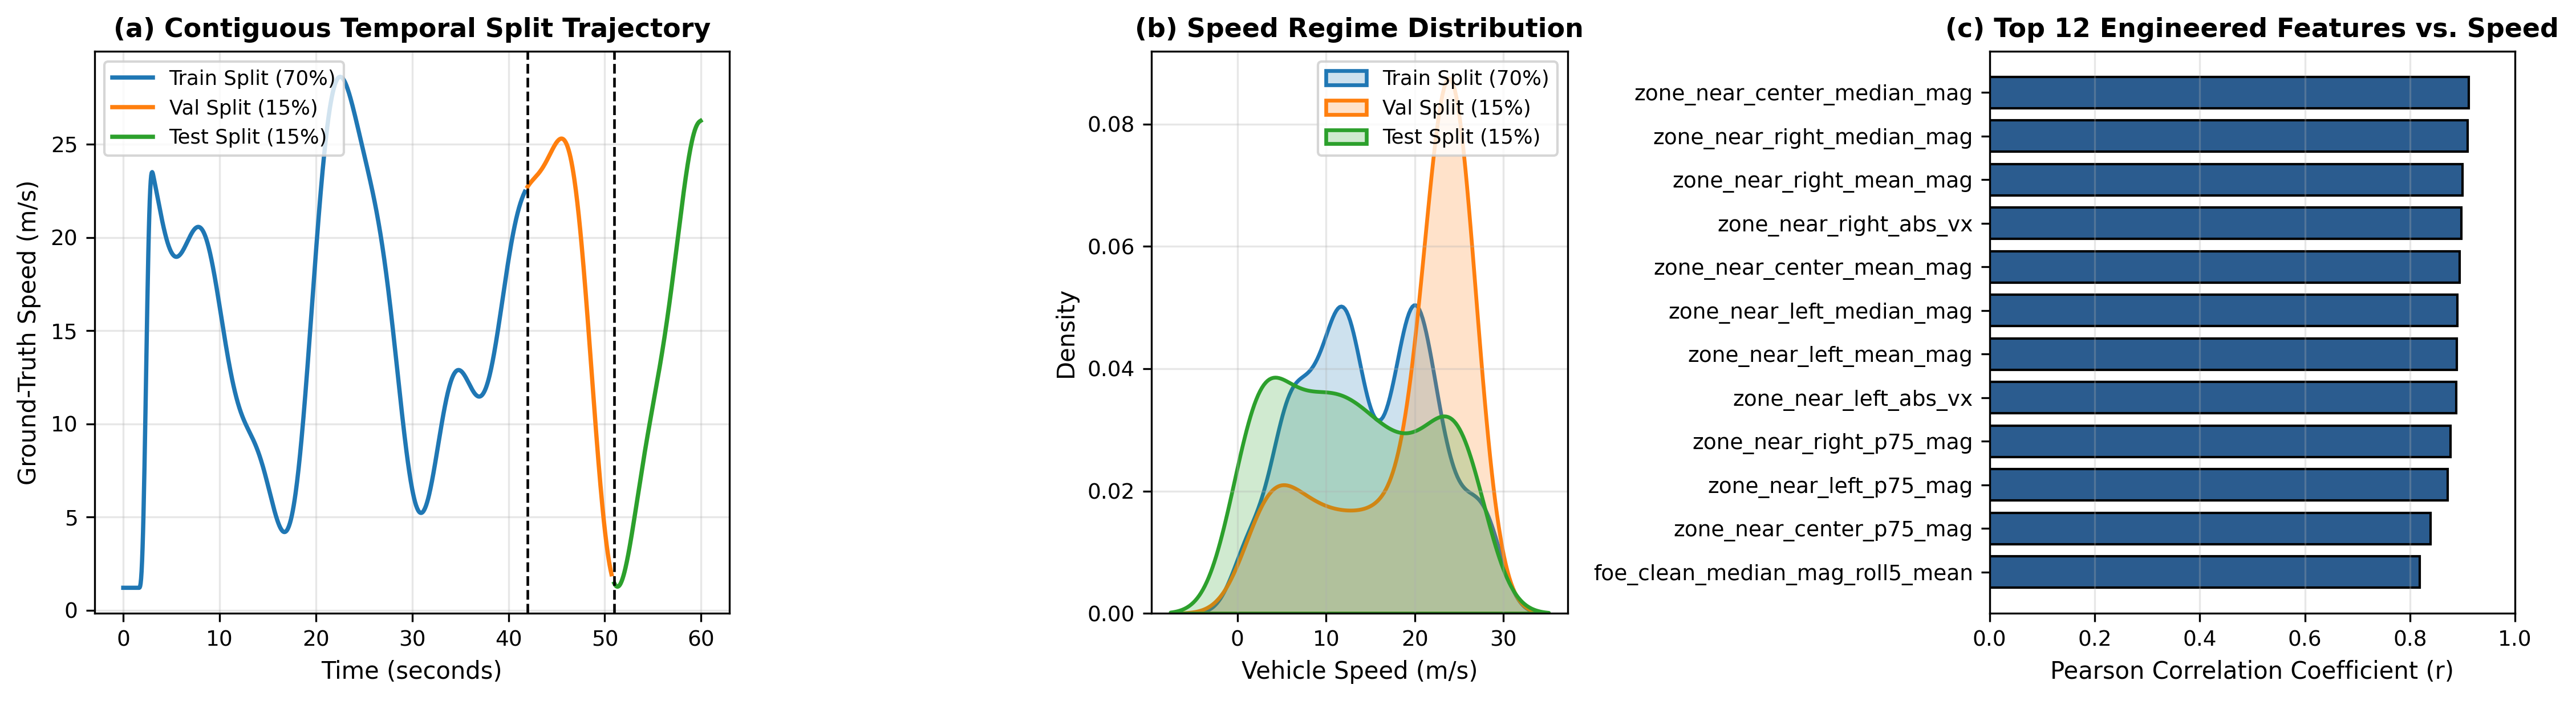
\includegraphics[width=0.98\linewidth]{figures/fig2_eda_speed_and_correlations.png}
  \captionof{figure}{Chronological Train/Val/Test velocity splits, speed density, and top feature Pearson correlations ($r > 0.91$).}
\end{center}

\columnbreak

\section*{\textcolor{navyheader}{2. Physics-Informed Features \& Ablation}}
\begin{itemize}
  \item \textbf{5 Feature Groups ($d=166$):} (1) Trapezoidal road ROI masking sky/hood; (2) FOE singularity exclusion + radial projection $v_r$; (3) Inverse-perspective depth scaling $\tilde{v}_y = v_y/((y-y_0)/H)^2$; (4) $3\times 3$ multi-zone grid order statistics; (5) Sparse LK + causal rolling kinematics.
  \item \textbf{Regularization + 1D Kalman Filter:} Gram matrix condition number $\kappa(\boldsymbol{\Phi}^\top\boldsymbol{\Phi}) = 4.79\times 10^{28}$ is stabilized via $\ell_2$ Ridge / $\ell_1$ Lasso and filtered by a 1D Constant-Acceleration Kalman Filter ($\mathbf{s}_t = [v_t, a_t]^\top$).
\end{itemize}

\begin{center}
  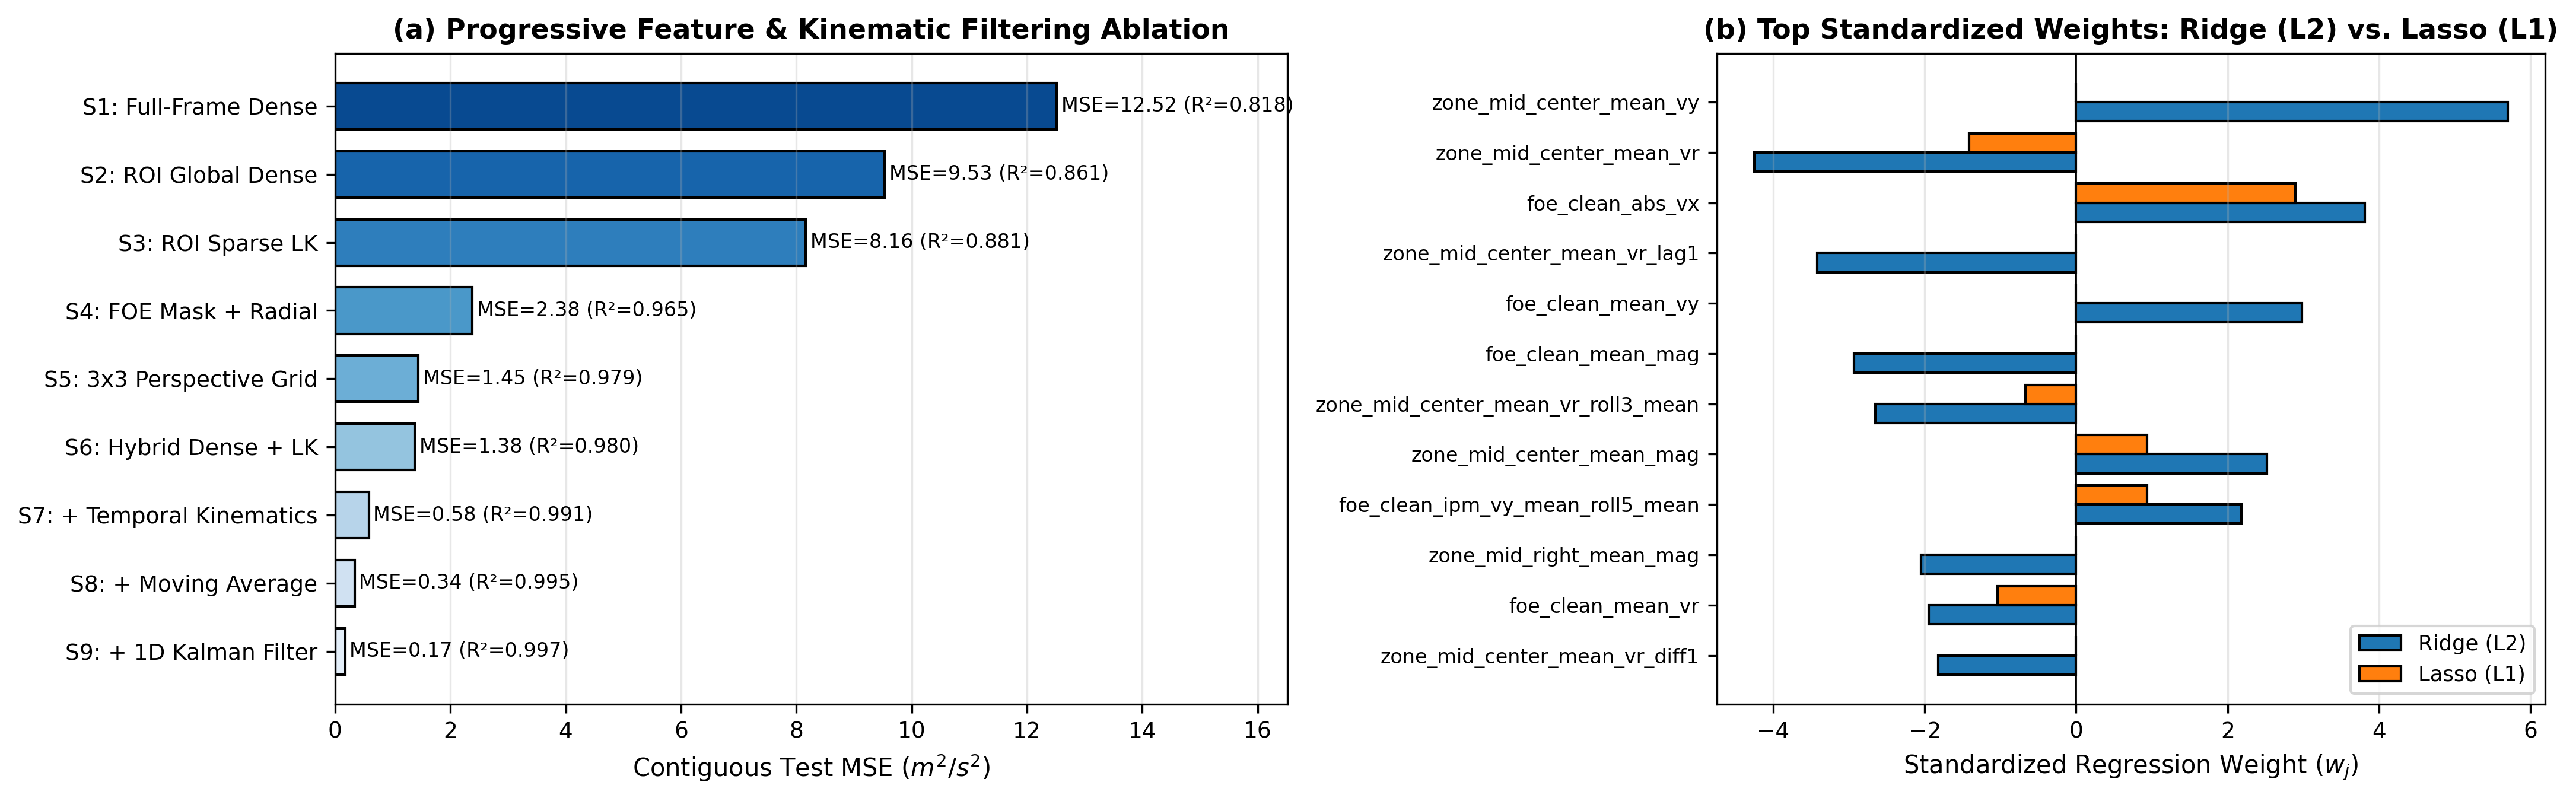
\includegraphics[width=0.98\linewidth]{figures/fig4_ablation_and_regularization.png}
  \captionof{figure}{9-stage progressive ablation ($98.6\%$ MSE reduction from S1 to S9) and standardized Ridge ($\ell_2$) vs.\ Lasso ($\ell_1$) weights.}
\end{center}

\begin{center}
  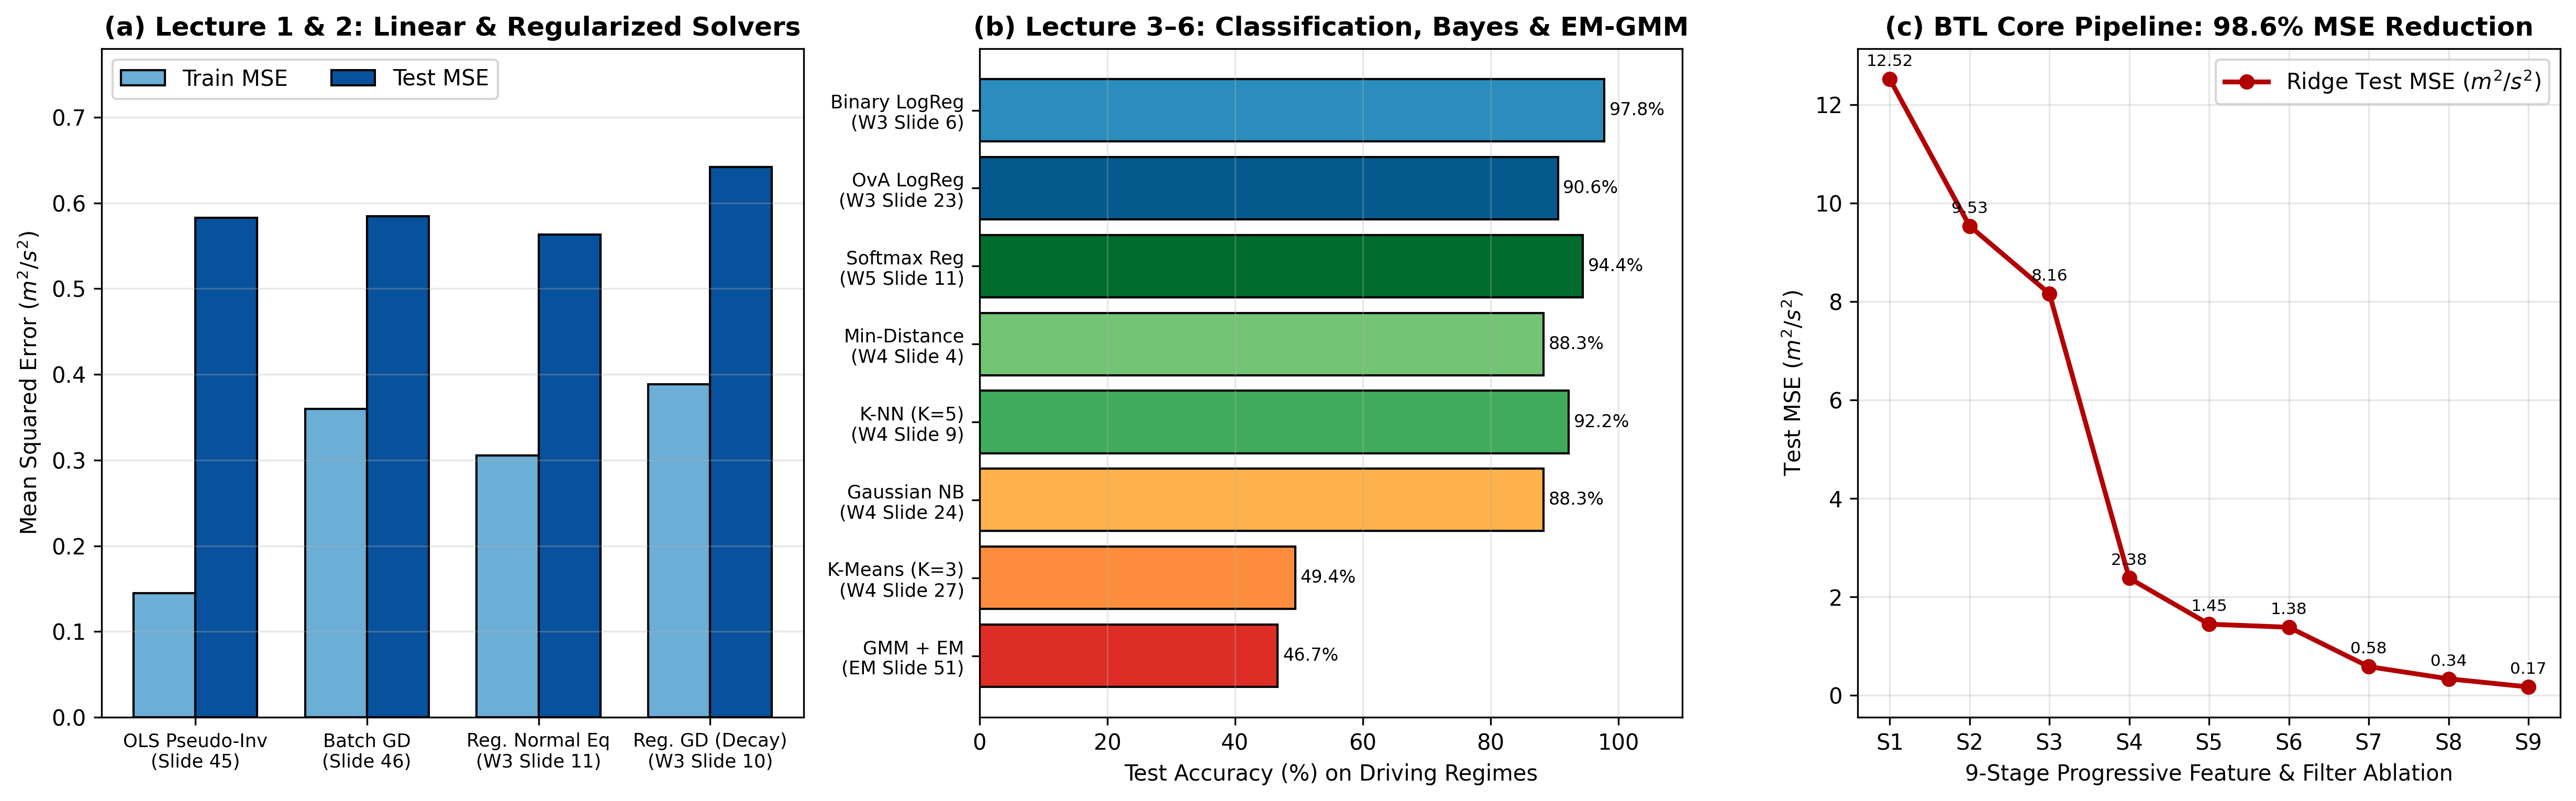
\includegraphics[width=0.98\linewidth]{figures/fig6_theory_alignment_benchmark.png}
  \captionof{figure}{CS229 Theory Alignment: Linear/Regularized solvers, Logistic/Softmax/Bayes/EM-GMM regime diagnostics, and ablation curve.}
\end{center}

\columnbreak

\section*{\textcolor{navyheader}{3. Trajectory Tracking \& Error Slicing}}
\begin{center}
  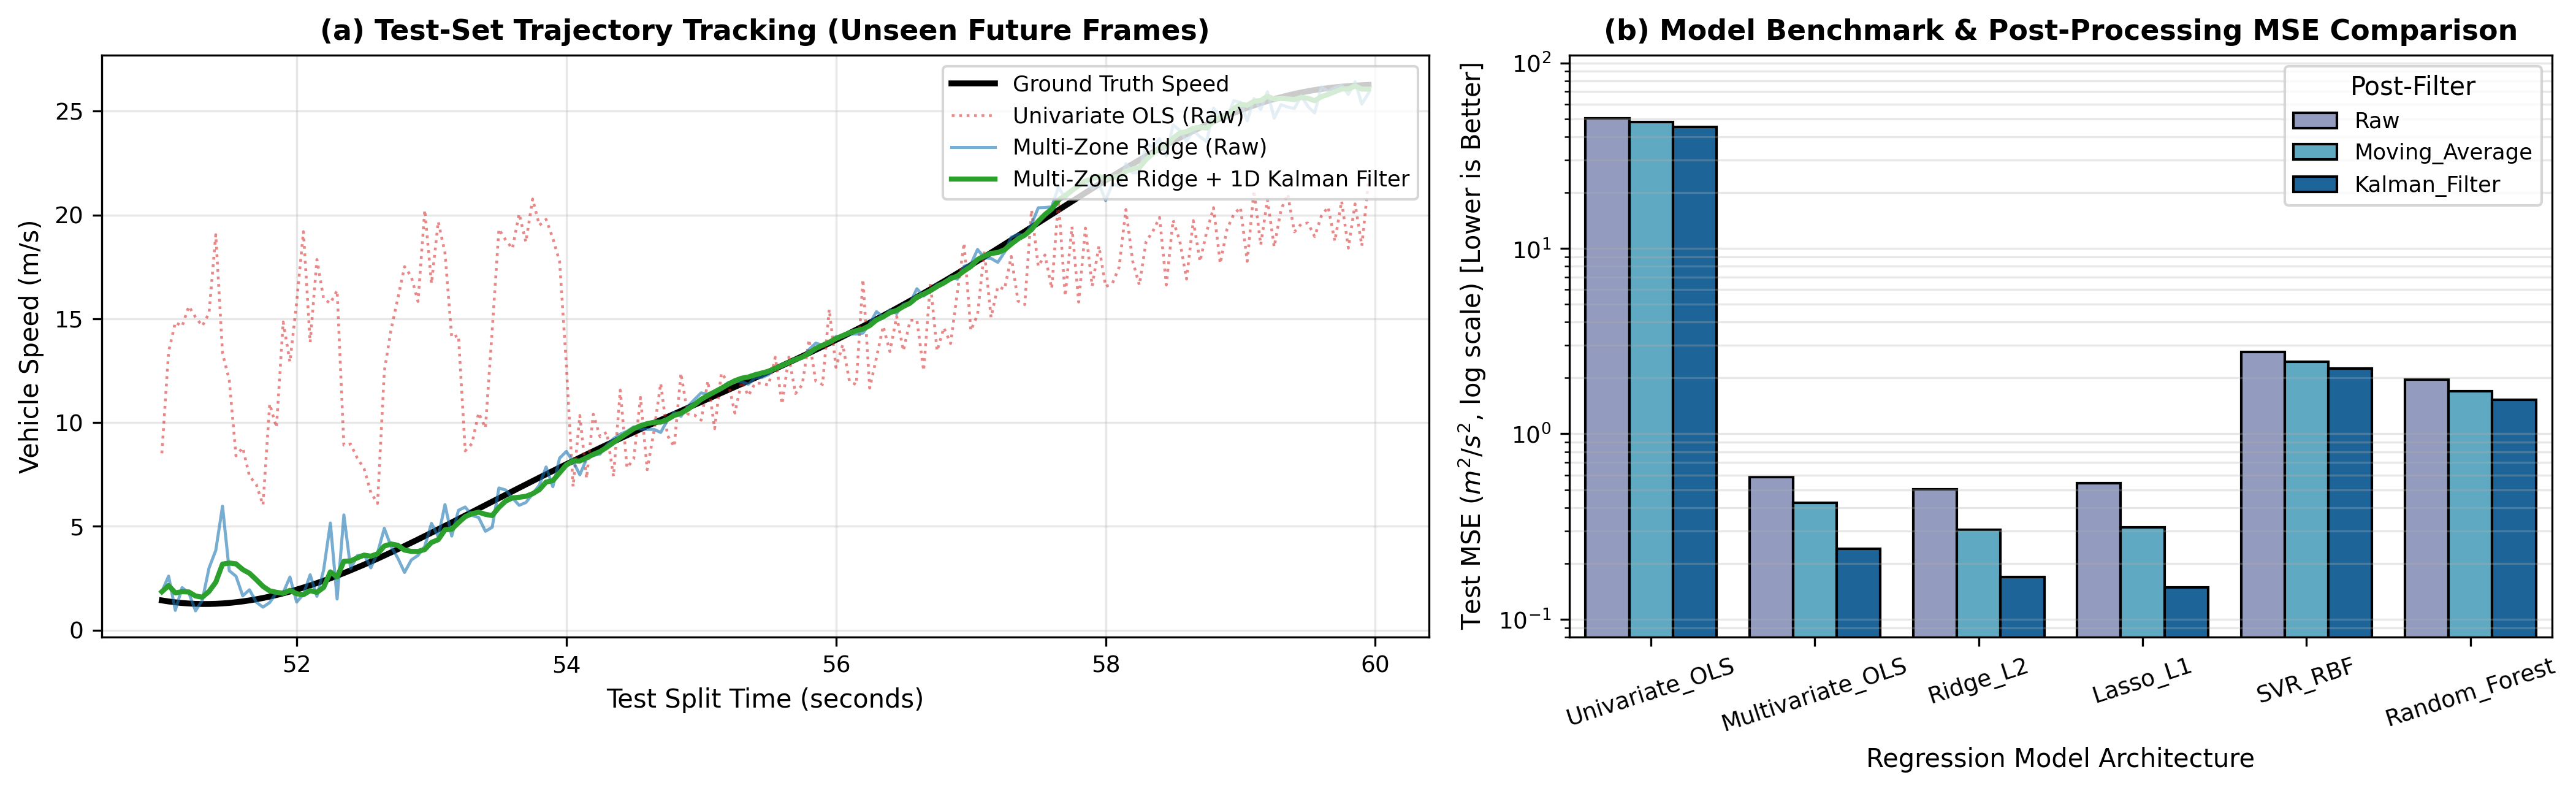
\includegraphics[width=0.98\linewidth]{figures/fig3_model_comparison_and_trajectories.png}
  \captionof{figure}{Unseen contiguous test-set velocity tracking and multi-model log-MSE comparison.}
\end{center}

\begin{center}
  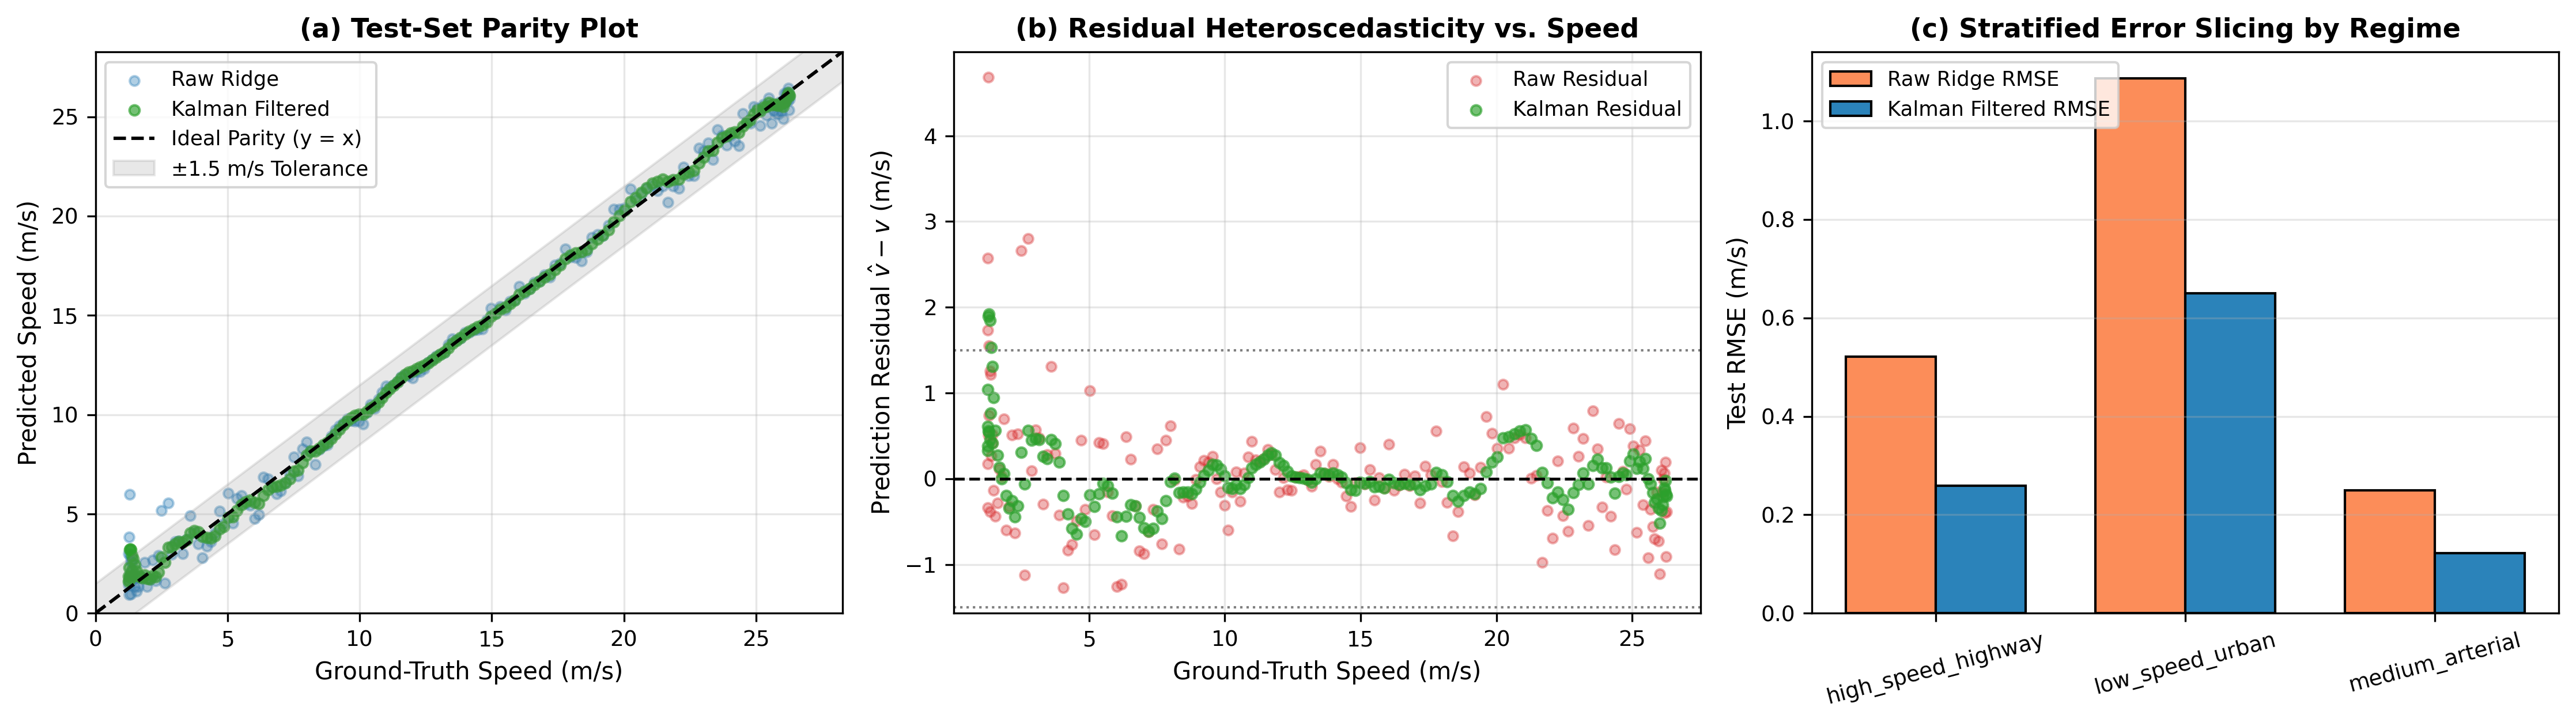
\includegraphics[width=0.98\linewidth]{figures/fig5_error_analysis_and_residuals.png}
  \captionof{figure}{Test parity plot, residual heteroscedasticity vs.\ speed, and stratified RMSE across driving regimes.}
\end{center}

\begin{center}
\small
\begin{tabular}{llcccc}
\toprule
\textbf{Model} & \textbf{Filter} & \textbf{Test MSE} & \textbf{RMSE} & \textbf{MAE} & \textbf{$R^2$} \\
\midrule
Univariate OLS & Raw & 50.385 & 7.098 & 5.460 & 0.2665 \\
RBF-SVR ($C=10$) & Kalman & 2.242 & 1.497 & 0.842 & 0.9674 \\
Random Forest & Kalman & 1.531 & 1.237 & 0.716 & 0.9777 \\
Multivariate OLS & Raw & 0.583 & 0.763 & 0.457 & 0.9915 \\
Ridge ($\alpha=0.1$) & Raw & 0.503 & 0.709 & 0.456 & 0.9927 \\
\textbf{Ridge ($\alpha=0.1$)} & \textbf{1D Kalman} & \textbf{0.168} & \textbf{0.410} & \textbf{0.266} & \textbf{0.9975} \\
\textbf{Lasso ($\alpha=0.005$)} & \textbf{1D Kalman} & \textbf{0.149} & \textbf{0.386} & \textbf{0.280} & \textbf{0.9978} \\
\bottomrule
\end{tabular}
\end{center}

\end{multicols}
\end{document}
